\chapter{Problem Statement and Proposed Approach}

% =============================
\section{Problem Statement}
Since the introduction of the Transformer architecture, the quality of language models has drastically increased \cite{devlin2018bert, radford2018improving}. They are now utilized in numerous downstream applications such as chatbots for medical purposes and an interactive \textit{Dungeons \& Dragons} hosted by an AI \cite{aidungeon}. In short, language models have become a commodity that nearly anyone can use for services that require some sort of natural language processing. 

Yet, language models are basically black boxes to us. Because of the enormous size of the support of these models, the learned probability distribution over natural language strings is difficult to analyze and therefore we have no idea what exactly goes on inside. We train language models on large amounts of text scraped from web sources and it is difficult to know what bias those large datasets might induce. For example, researchers have shown that the models trained by certain texts encode social biases, such as religion, gender and race \cite{abid2021persistent}. Through various probing techniques we can take a peak at some properties, which can then be influenced by tweaking parameters, dataset augmentation and "creating pseudo-training data to encode those biases" \cite{MarasovicGradient2018NLP} - but this is the extent of it. According to Ricardo Baeza-Yates from the Institute for Experimental AI \cite{lmfail}, the three major limitations of language models are "\textit{unequal language resources}", "\textit{the bias from learned text}" and "\textit{the lack of semantic understanding at an extreme cost}". This shows that we need better tools to understand what exactly our language models learn in order to be able to train and use them accordingly. 
% =============================
\section{Proposed Approach}
We propose an approach for looking at the semantic spaces---as defined by topics---learned by these language models. In order to understand some of the model's inductive biases, we look at those semantic spaces and at how they differ from the ones the corpora models were trained on. Inductive biases are biases built into the model that are not based on the training data.

We utilize a known technique from natural language processing: the topic model. Through topic model techniques we cluster the generated output from certain language models as well as the corpus they are trained on (see fig. \ref{fig:generationexample} and \ref{fig:analyzing_pipeline}).  Finally, we compare those two topic models using our own designed metric. 
\begin{figure}[H]
    \centering
    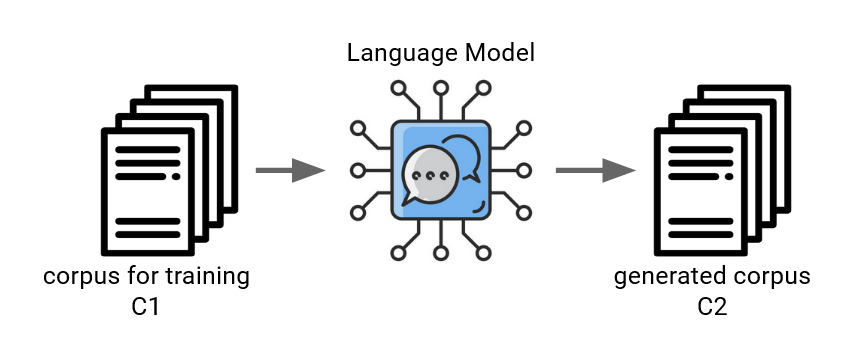
\includegraphics[width=0.7\textwidth]{figures/generationexample}
    \caption{Illustration of the correlation between corpus $C1$ and $C2$.}
    \label{fig:generationexample}
\end{figure}
\begin{figure}[H]
    \centering
    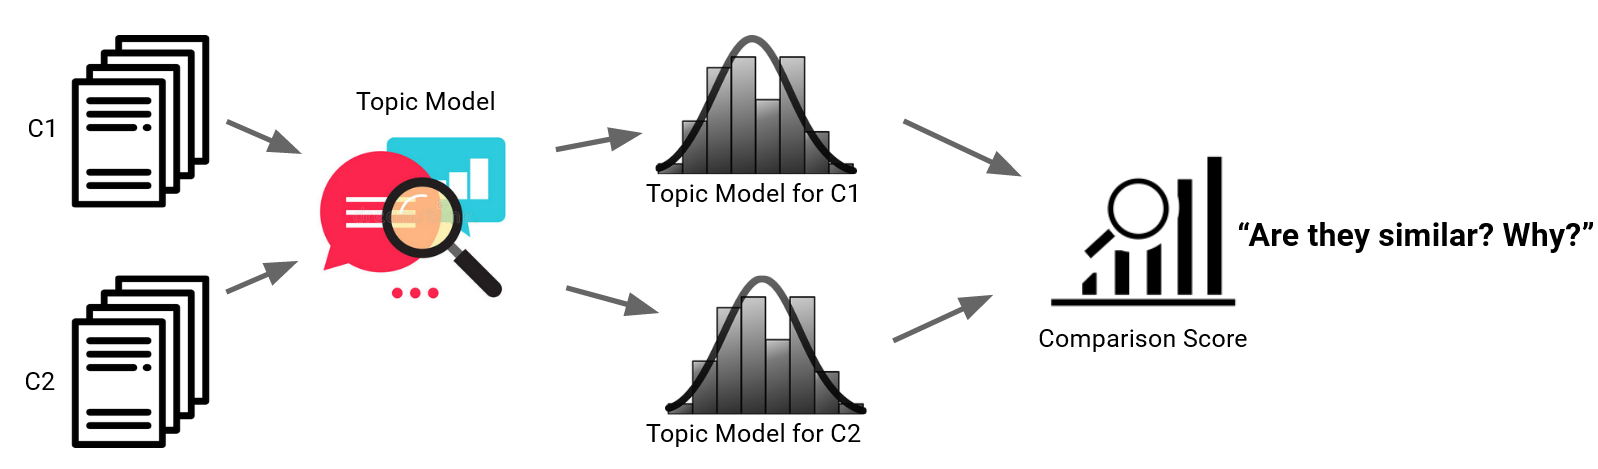
\includegraphics[width=1.0\textwidth]{figures/analyzing_pipeline}
    \caption{Illustration of the analyzation pipeline. $C1$ and $C2$ are different corpora.}
    \label{fig:analyzing_pipeline}
\end{figure}

Specifically, we train a GPT-2 \cite{gpt-2} and a Transformer-XL \cite{transformer-xl} model on the full Wikitext103 \cite{wikitext} corpus ($C1$). Then, we use latent Dirichlet allocation (LDA) \cite{blei2003latent} and neural LDA \cite{neuralLDA} to train topic models for $C1$ and $C2$, where $C2$ is the generated output from our trained language models. 

For us to be able to gain some insight, we need more data than only from comparing two language models and two topic models. Therefore, when generating a corpus from a language model, we compare different sampling techniques with each other (ancestral sampling, Top-P sampling \cite{holtzman2019curious} and Typical sampling \cite{meister2022typical}). For the topic models we use different topic sizes ($\{2, 3, 5, 10, 20, 50, 100\}$) and additional corpora (Wikitext103 \cite{wikitext}, ArXiv Metadata \cite{arxiv}, the original GPT-2 model \cite{gpt2model}, the original Transformer XL model \cite{trafoxlmodel}). 

We know topic models use the words from tokenized text to create topics (probability distributions over words). Thus, we additionally consider the possibility of word combinations, e.g. \texttt{machine\_learning},  \texttt{deep\_neural\_network} and so on. This means that we compare the influence of bigrams (two word combinations) and trigrams (three word combinations) in our text instead of only using single words for the creation of topic models.

If we want to compare two topic models with each other, their vocabulary has to be exactly the same. The vocabulary contains all words of the training text for the topic model after the tokenization process. We decide between taking the intersection and the union of the two vocabularies. As we do not know the impact of taking one over the other, we evaluate both in our research. 

To analyze the quality and stability of our topic models, we employ the coherence score $C_v$ (see sec. \ref{sec:coherence}). For comparing two topic models, we design our own metric. First, we calculate the probability of every topic in both corpora. Then, we calculate the distance matrix using the Jensen-Shannon distance (see sec. \ref{sec:diffmet}), weigh the value of the two closest topics for each row and column by the respective topic probability, and sum them up. 